\chapter{Mesure de la carte principale}

\section{Introduction}
La mesure de la carte principale permet de déterminer plusieurs points des hypothèses émise tel que

\subsection{Objéctif de la mesure}
Les objéctif de la mesure sont :

\begin{itemize}
    \item Déterminer si la carte est correctement alimenté.
    \item Vérifier que les capteurs de courants fonctionne correctement.
    \item Vérifier que les capteurs de positions fonctionne correctement
    \item Déterminer le besoin d'une nouvelle calibration des capteurs de positons.
\end{itemize}

\section{Vérification de la charge du condensateur}
Le condensateur a été vérifié afin de comparer le résultat obtenu à celui de Thomas Freyche, illustré dans la figure \ref{fig:ResFreycheCapa} :

\begin{figure}[H]
    \centering
    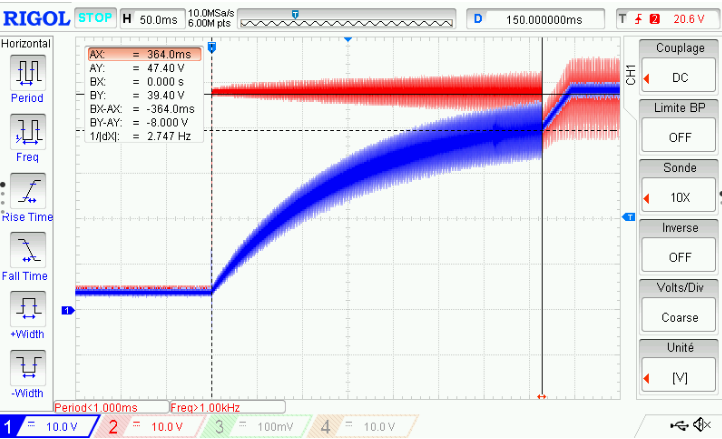
\includegraphics[width=0.75\linewidth]{assets/Chap3/Result_Freyche_Capa.png}
    \caption{Résultat de la mesure du condensateur du rapport de Thomas Freyche \cite{Freyche}}
    \label{fig:ResFreycheCapa}
\end{figure}

Lors de la mesure effectuée pour ce travail, un résultat identique a été obtenu, comme le montre la figure \ref{fig:ResCanCapa} :

\begin{figure}[H]
    \centering
    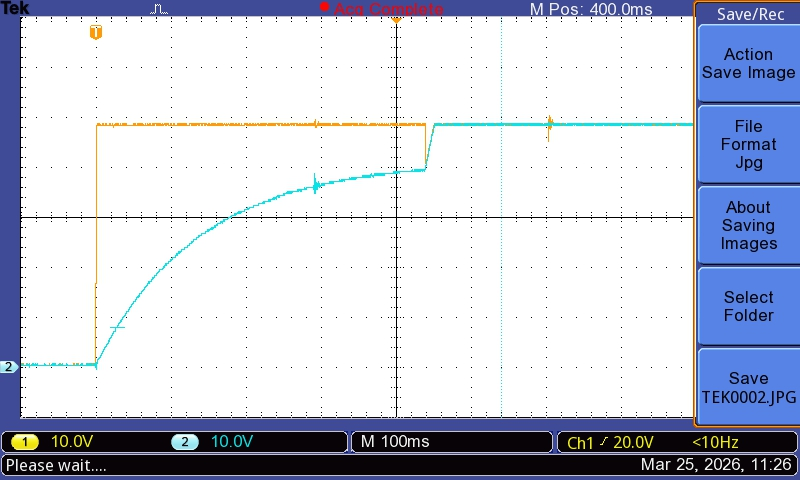
\includegraphics[width=0.75\linewidth]{assets/Chap3/MesureCondoCan.JPG}
    \caption{Résultat de la mesure du condensateur personnel}
    \label{fig:ResCanCapa}
\end{figure}

Cela vient prouver le bon fonctionnement du circuit de précharge.

\section{Mesure des régulateurs}

Cette section traite des mesures réalisées sur les régulateurs de la carte principale. Ces composants assurent l'alimentation correcte de l'intégralité du système.\\

Le convertisseur 24 V présente les résultats consignés dans le tableau \ref{tab:reg_24v_48v} :

\begin{table}[H]
    \centering
    \resizebox{\textwidth}{!}{%
        \begin{tabular}{|c|l|c|c|c|c|c|}
            \hline
            \multicolumn{7}{|c|}{\textbf{Régulateurs 24V et entrée 48V (PS1)}}                                                                                                                                                              \\ \hline
            N°  & \multicolumn{1}{c|}{Mesure}          & Point de mesure & \begin{tabular}[c]{@{}c@{}}Valeur théorique\\ {[}V{]}\end{tabular} & \begin{tabular}[c]{@{}c@{}}Valeur\\ mesurée {[}V{]}\end{tabular} & Erreur & Erreur {[}\%]{} \\ \hline
            1.a & Entrée des 48V                       & Bornie d'entrée & 48                                                                 & 48.05                                                            & 0.05   & 0.10            \\ \hline
            1.b & Tension après le switch de précharge & TP4             & 48                                                                 & 48.04                                                            & 0.04   & 0.08            \\ \hline
            2.a & Sortie du régulateur 24V             & TP6 et TP8      & 24                                                                 & 23.85                                                            & 0.15   & 0.62            \\ \hline
        \end{tabular}%
    }
    \caption{Mesures sur les régulateurs 24V et l'entrée 48V (PS1)}
    \label{tab:reg_24v_48v}
\end{table}

Le régulateur de 15 V présente les résultats consignés dans le tableau \ref{tab:reg_15v} :

\begin{table}[H]
    \centering
    \resizebox{\textwidth}{!}{%
        \begin{tabular}{|c|l|c|c|c|c|c|}
            \hline
            \multicolumn{7}{|c|}{\textbf{Régulateurs 15V (PS2)}}                                                                                                                                                                      \\ \hline
            N°  & \multicolumn{1}{c|}{Mesure} & Point de mesure    & \begin{tabular}[c]{@{}c@{}}Valeur théorique\\ {[}V{]}\end{tabular} & \begin{tabular}[c]{@{}c@{}}Valeur\\ mesurée {[}V{]}\end{tabular} & Erreur & Erreur {[}\%]{} \\ \hline
            1.a & Entrée des 24V              & Côté C12 de la C13 & 24                                                                 & 23.07                                                            & 0.93   & 3.88            \\ \hline
            2.a & Sortie du régulateur 15V    & TP1                & 15                                                                 & 14.95                                                            & 0.05   & 0.333           \\ \hline
        \end{tabular}%
    }
    \caption{Mesures sur le régulateur 15V (PS2)}
    \label{tab:reg_15v}
\end{table}

Le régulateur de 5 V présente les résultats consignés dans le tableau \ref{tab:reg_5v} :

\begin{table}[H]
    \centering
    \resizebox{\textwidth}{!}{%
        \begin{tabular}{|c|l|c|c|c|c|c|}
            \hline
            \multicolumn{7}{|c|}{\textbf{Régulateurs 5V (IC1)}}                                                                                                                                                                    \\ \hline
            N°  & \multicolumn{1}{c|}{Mesure} & Point de mesure & \begin{tabular}[c]{@{}c@{}}Valeur théorique\\ {[}V{]}\end{tabular} & \begin{tabular}[c]{@{}c@{}}Valeur\\ mesurée {[}V{]}\end{tabular} & Erreur & Erreur {[}\%]{} \\ \hline
            1.a & Entrée des 24V              & Pin 1 IC1       & 24                                                                 & 23.86                                                            & 0.14   & 0.583           \\ \hline
            2.a & Sortie du régulateur 5V     & L2 côté condo   & 5                                                                  & 4.989                                                            & 0.011  & 0.220           \\ \hline
            2.b & Après l'inducteur L2        & TP2             & 5                                                                  & 4.987                                                            & 0.013  & 0.260           \\ \hline
        \end{tabular}%
    }
    \caption{Mesures sur les régulateurs 5V (IC1)}
    \label{tab:reg_5v}
\end{table}

Le régulateur de 3,3 V présente les résultats consignés dans le tableau \ref{tab:reg_3_3v} :

\begin{table}[H]
    \centering
    \resizebox{\textwidth}{!}{%
        \begin{tabular}{|c|l|c|c|c|c|c|}
            \hline
            \multicolumn{7}{|c|}{\textbf{Régulateurs 3.3V (U6)}}                                                                                                                                                                   \\ \hline
            N°  & \multicolumn{1}{c|}{Mesure} & Point de mesure & \begin{tabular}[c]{@{}c@{}}Valeur théorique\\ {[}V{]}\end{tabular} & \begin{tabular}[c]{@{}c@{}}Valeur\\ mesurée {[}V{]}\end{tabular} & Erreur & Erreur {[}\%]{} \\ \hline
            1.a & Entrée des 5V               & J5 pin 2        & 5                                                                  & 4.982                                                            & 0.018  & 0.360           \\ \hline
            2.a & Sortie du régulateur 3.3V   & TP5             & 3.3                                                                & 3.296                                                            & 0.004  & 0.121           \\ \hline
        \end{tabular}%
    }
    \caption{Mesures sur les régulateurs 3.3V (U6)}
    \label{tab:reg_3_3v}
\end{table}

Le régulateur de 0,5 V présente les résultats consignés dans le tableau \ref{tab:reg_0_5v} :

\begin{table}[H]
    \centering
    \resizebox{\textwidth}{!}{%
        \begin{tabular}{|c|l|c|c|c|c|c|}
            \hline
            \multicolumn{7}{|c|}{\textbf{Régulateurs 0.5V (U5)}}                                                                                                                                                                   \\ \hline
            N°  & \multicolumn{1}{c|}{Mesure} & Point de mesure & \begin{tabular}[c]{@{}c@{}}Valeur théorique\\ {[}V{]}\end{tabular} & \begin{tabular}[c]{@{}c@{}}Valeur\\ mesurée {[}V{]}\end{tabular} & Erreur & Erreur {[}\%]{} \\ \hline
            1.a & Entrée des 24V              & C18 côté U6     & 5                                                                  & 4.981                                                            & 0.019  & 0.380           \\ \hline
            2.a & Sortie du régulateur 15V    & TP3             & 0.5                                                                & 0.4982                                                           & 0.002  & 0.360           \\ \hline
        \end{tabular}%
    }
    \caption{Mesures sur les régulateurs 0.5V (U5)}
    \label{tab:reg_0_5v}
\end{table}

\subsection{Analyse des résultats}
Les différents régulateurs présentés ci-dessus fonctionnent de manière nominale. Les tensions fournies sont conformes aux spécifications des constructeurs, ce qui garantit une alimentation stable pour l'ensemble de la carte.

Une anomalie a néanmoins été détectée sur le convertisseur 24 V lors des essais. Une broche mal soudée provoquait l'apparition d'arcs électriques sous le circuit imprimé. Ce module devra donc faire l'objet d'une attention particulière en cas de futurs dysfonctionnements électriques. Après la reprise de la soudure, le phénomène a été éliminé.

\section{Mesure des capteurs de courants}
Cette section traite des différentes mesures réalisées afin de vérifier le comportement des capteurs de courant.

Dans un premier temps, une évaluation globale du bon fonctionnement des composants situés entre le capteur de courant et l'étage de réception des données par l'ADC a été effectuée.

Par la suite, le chariot a été soulevé uniquement du côté avant ou arrière. Cette manipulation permet de modifier la répartition de la force de pesanteur et d'alourdir localement la charge sur les inducteurs concernés. En fonctionnement nominal, la force électromécanique générée doit compenser cette charge pour maintenir la lévitation. La sustentation simultanée sur les quatre inducteurs n'étant pas exploitable au moment des tests, l'analyse s'est concentrée sur le soulèvement isolé de l'avant ou de l'arrière. L'application de ces charges connues offre la possibilité de calculer théoriquement le courant requis à partir de la force appliquée et des valeurs nominales de l'entrefer.\\

\subsection{Mesure des circuits de conditionnement des capteurs de courants}

Les mesures globales des circuits de conditionnement sont présentées dans les tableaux \ref{tab:cond_courant_1} et \ref{tab:cond_courant_2} :


\begin{table}[H]
    \centering
    \resizebox{\textwidth}{!}{%
        \begin{tabular}{|c|c|c|c|c|c|c|}
            \hline
            \multicolumn{7}{|c|}{\textbf{Vérification général des conditionneurs de courant}}                                                                                                                                                                                                                                                             \\ \hline
            N°  & Mesure                                                                & \begin{tabular}[c]{@{}c@{}}Point de\\ mesure\end{tabular}   & \begin{tabular}[c]{@{}c@{}}Valeur théorique\\ {[}V{]}\end{tabular} & \begin{tabular}[c]{@{}c@{}}Valeur mesurée\\ {[}V{]}\end{tabular} & Erreur                                  & Erreur {[}\%{]} \\ \hline
            1.a & \begin{tabular}[c]{@{}c@{}}Alimentation de\\ l'AOP U1\_4\end{tabular} & U1\_4 pin 8                                                 & 5                                                                  & 4.989                                                            & 0.0110                                  & 0.2200          \\ \hline
            1.b & \begin{tabular}[c]{@{}c@{}}Alimentation de\\ l'AOP U2\_4\end{tabular} & U2\_4 pin 8                                                 & 3.3                                                                & 3.296                                                            & 0.0040                                  & 0.1212          \\ \hline
            1.c & \begin{tabular}[c]{@{}c@{}}Sortie du capteur\\ 1\end{tabular}         & \begin{tabular}[c]{@{}c@{}}R3\_4 côté\\ droite\end{tabular} & 0.625..4.375                                                       & 2.933                                                            & \multicolumn{2}{c|}{\multirow{3}{*}{-}}                   \\ \cline{1-5}
            1.d & \begin{tabular}[c]{@{}c@{}}Sortie de l'AOP\\ U1\_4\end{tabular}       & U2\_4 pin 5                                                 & 0.5..3.5                                                           & 1.173                                                            & \multicolumn{2}{c|}{}                                     \\ \cline{1-5}
            1.e & \begin{tabular}[c]{@{}c@{}}Sortie de l'AOP\\ U2\_4\end{tabular}       & TP9\_4                                                      & 0..3                                                               & 1.888                                                            & \multicolumn{2}{c|}{}                                     \\ \hline
            2.a & \begin{tabular}[c]{@{}c@{}}Alimentation de\\ l'AOP U1\_1\end{tabular} & U1\_1 pin 8                                                 & 5                                                                  & 4.984                                                            & 0.0160                                  & 0.3200          \\ \hline
            2.b & \begin{tabular}[c]{@{}c@{}}Alimentation de\\ l'AOP U2\_1\end{tabular} & U2\_1 pin 8                                                 & 3.3                                                                & 3.296                                                            & 0.0040                                  & 0.1212          \\ \hline
            2.c & \begin{tabular}[c]{@{}c@{}}Sortie du capteur\\ 2\end{tabular}         & \begin{tabular}[c]{@{}c@{}}R9\_1 côté\\ gauche\end{tabular} & 0.625..4.375                                                       & 2.872                                                            & \multicolumn{2}{c|}{\multirow{3}{*}{-}}                   \\ \cline{1-5}
            2.d & \begin{tabular}[c]{@{}c@{}}Sortie de l'AOP\\ U1\_1\end{tabular}       & U2\_1 pin 5                                                 & 0.5..3.5                                                           & 1.139                                                            & \multicolumn{2}{c|}{}                                     \\ \cline{1-5}
            2.e & \begin{tabular}[c]{@{}c@{}}Sortie de l'AOP\\ U2\_1\end{tabular}       & TP9\_1                                                      & 0..3                                                               & 1.736                                                            & \multicolumn{2}{c|}{}                                     \\ \hline
        \end{tabular}%
    }
    \caption{Vérification générale des conditionneurs de courant (Capteurs 1 et 2)}
    \label{tab:cond_courant_1}
\end{table}

\begin{table}[h!]
    \centering
    \resizebox{\textwidth}{!}{%
        \begin{tabular}{|c|c|c|c|c|c|c|}
            \hline
            \multicolumn{7}{|c|}{\textbf{Vérification général des conditionneurs de courant}}                                                                                                                                                                                                                                                             \\ \hline
            N°  & Mesure                                                                & \begin{tabular}[c]{@{}c@{}}Point de\\ mesure\end{tabular}   & \begin{tabular}[c]{@{}c@{}}Valeur théorique\\ {[}V{]}\end{tabular} & \begin{tabular}[c]{@{}c@{}}Valeur mesurée\\ {[}V{]}\end{tabular} & Erreur                                  & Erreur {[}\%{]} \\ \hline
            3.a & \begin{tabular}[c]{@{}c@{}}Alimentation de\\ l'AOP U1\_3\end{tabular} & U1\_3 pin 8                                                 & 5                                                                  & 4.985                                                            & 0.0150                                  & 0.3000          \\ \hline
            3.b & \begin{tabular}[c]{@{}c@{}}Alimentation de\\ l'AOP U2\_3\end{tabular} & U2\_3 pin 8                                                 & 3.3                                                                & 3.296                                                            & 0.0040                                  & 0.1212          \\ \hline
            3.c & \begin{tabular}[c]{@{}c@{}}Sortie du capteur\\ 3\end{tabular}         & \begin{tabular}[c]{@{}c@{}}R9\_3 côté\\ droite\end{tabular} & 0.625..4.375                                                       & 2.485                                                            & \multicolumn{2}{c|}{\multirow{3}{*}{-}}                   \\ \cline{1-5}
            3.d & \begin{tabular}[c]{@{}c@{}}Sortie de l'AOP\\ U1\_3\end{tabular}       & U2\_3 pin 5                                                 & 0.5..3.5                                                           & 0.996                                                            & \multicolumn{2}{c|}{}                                     \\ \cline{1-5}
            3.e & \begin{tabular}[c]{@{}c@{}}Sortie de l'AOP\\ U2\_3\end{tabular}       & TP9\_3                                                      & 0..3                                                               & 1.532                                                            & \multicolumn{2}{c|}{}                                     \\ \hline
            4.a & \begin{tabular}[c]{@{}c@{}}Alimentation de\\ l'AOP U1\_2\end{tabular} & U1\_2 pin 8                                                 & 5                                                                  & 4.984                                                            & 0.0160                                  & 0.3200          \\ \hline
            4.b & \begin{tabular}[c]{@{}c@{}}Alimentation de\\ l'AOP U2\_2\end{tabular} & U2\_2 pin 8                                                 & 3.300                                                              & 3.296                                                            & 0.0040                                  & 0.1212          \\ \hline
            4.c & \begin{tabular}[c]{@{}c@{}}Sortie du capteur\\ 4\end{tabular}         & \begin{tabular}[c]{@{}c@{}}R9\_2 côté\\ gauche\end{tabular} & 0.625..4.375                                                       & 2.498                                                            & \multicolumn{2}{c|}{\multirow{3}{*}{-}}                   \\ \cline{1-5}
            4.d & \begin{tabular}[c]{@{}c@{}}Sortie de l'AOP\\ U1\_2\end{tabular}       & U2\_2 pin 5                                                 & 0.5..3.5                                                           & 0.999                                                            & \multicolumn{2}{c|}{}                                     \\ \cline{1-5}
            4.e & \begin{tabular}[c]{@{}c@{}}Sortie de l'AOP\\ U2\_2\end{tabular}       & TP9\_2                                                      & 0..3                                                               & 1.545                                                            & \multicolumn{2}{c|}{}                                     \\ \hline
        \end{tabular}%
    }
    \caption{Vérification générale des conditionneurs de courant (Capteurs 3 et 4)}
    \label{tab:cond_courant_2}
\end{table}

\subsection{Mesure du courant sans ajout de poids}
Une première série de mesures a été réalisée sans ajout de masse afin d'établir des comparaisons entre les valeurs théoriques, les mesures par sonde de courant et les données acquises par l'ADC. Ces résultats sont consignés dans les tableaux \ref{tab:sans_poids_sonde}, \ref{tab:sans_poids_adc} et \ref{tab:sans_poids_comp} :

% --- Sans Poids - Partie 1 (Sonde) ---
\begin{table}[H]
    \centering
    \resizebox{\textwidth}{!}{%
        \begin{tabular}{|c|c|c|c|c|c|c|c|c|c|}
            \hline
            \multicolumn{10}{|c|}{\textbf{Sans poids}}                                                                                                                                                                                                                                                                                                                                                                                                                                                              \\ \hline
            Inducteur & \begin{tabular}[c]{@{}c@{}}Position\\ {[}m{]}\end{tabular} & L {[}H{]}                 & \begin{tabular}[c]{@{}c@{}}k\\ {[}m*A/N{]}\end{tabular} & \begin{tabular}[c]{@{}c@{}}Masse\\ {[}kg{]}\end{tabular} & \begin{tabular}[c]{@{}c@{}}Force\\ {[}N{]}\end{tabular} & \begin{tabular}[c]{@{}c@{}}Courant\\ théorique {[}A{]}\end{tabular} & \begin{tabular}[c]{@{}c@{}}Courant\\ mesuré {[}A{]}\end{tabular} & Erreur & \begin{tabular}[c]{@{}c@{}}Erreur\\ relatif {[}\%{]}\end{tabular} \\ \hline
            1         & \multirow{4}{*}{2.00E-03}                                  & \multirow{4}{*}{4.90E-03} & \multirow{4}{*}{4.90E-06}                               & \multirow{4}{*}{9.03}                                    & 89                                                      & 8.5                                                                 & 6.1                                                              & 2.4    & 28                                                                \\ \cline{1-1} \cline{6-10}
            2         &                                                            &                           &                                                         &                                                          & 89                                                      & 8.5                                                                 & 6.2                                                              & 2.3    & 28                                                                \\ \cline{1-1} \cline{6-10}
            3         &                                                            &                           &                                                         &                                                          & 89                                                      & 8.5                                                                 & 6.4                                                              & 2.1    & 25                                                                \\ \cline{1-1} \cline{6-10}
            4         &                                                            &                           &                                                         &                                                          & 89                                                      & 8.5                                                                 & 5.8                                                              & 2.7    & 31                                                                \\ \hline
        \end{tabular}%
    }
    \caption{Mesures de courant par sonde (Sans poids)}
    \label{tab:sans_poids_sonde}
\end{table}

% --- Sans Poids - Partie 2 (ADC) ---
\begin{table}[H]
    \centering
    \resizebox{\textwidth}{!}{%
        \begin{tabular}{|c|c|c|c|c|c|c|c|c|c|}
            \hline
            \multicolumn{10}{|c|}{\textbf{Sans poids}}                                                                                                                                                                                                                                                                                                                                                                                                                                                   \\ \hline
            Inducteur & \begin{tabular}[c]{@{}c@{}}Position\\ {[}m{]}\end{tabular} & L {[}H{]}                 & \begin{tabular}[c]{@{}c@{}}k\\ {[}m*A/N{]}\end{tabular} & \begin{tabular}[c]{@{}c@{}}Masse\\ {[}kg{]}\end{tabular} & \begin{tabular}[c]{@{}c@{}}Force\\ {[}N{]}\end{tabular} & \begin{tabular}[c]{@{}c@{}}Courant\\ théorique {[}A{]}\end{tabular} & \begin{tabular}[c]{@{}c@{}}ADC\\ {[}A{]}\end{tabular} & Erreur & \begin{tabular}[c]{@{}c@{}}Erreur\\ relatif {[}\%{]}\end{tabular} \\ \hline
            1         & \multirow{4}{*}{2.00E-03}                                  & \multirow{4}{*}{4.90E-03} & \multirow{4}{*}{4.90E-06}                               & \multirow{4}{*}{9.026}                                   & 88.5                                                    & 8.50                                                                & 6.79                                                  & 1.717  & 20.19                                                             \\ \cline{1-1} \cline{6-10}
            2         &                                                            &                           &                                                         &                                                          & 88.5                                                    & 8.50                                                                & 6.45                                                  & 2.056  & 24.2                                                              \\ \cline{1-1} \cline{6-10}
            3         &                                                            &                           &                                                         &                                                          & 88.5                                                    & 8.50                                                                & 6.54                                                  & 1.964  & 23.1                                                              \\ \cline{1-1} \cline{6-10}
            4         &                                                            &                           &                                                         &                                                          & 88.5                                                    & 8.50                                                                & 6.02                                                  & 2.48   & 29.2                                                              \\ \hline
        \end{tabular}%
    }
    \caption{Mesures de courant par ADC (Sans poids)}
    \label{tab:sans_poids_adc}
\end{table}

\begin{table}[H]
    \centering
    \begin{tabular}{|c|c|c|c|}
        \hline
        \multicolumn{4}{|c|}{\textbf{Sans poids}}        \\ \hline
        Inducteur & ADC {[}A{]} & Sonde {[}A{]} & Erreur \\ \hline
        1         & 6.79        & 6.08          & 0.71   \\ \hline
        2         & 6.45        & 6.16          & 0.29   \\ \hline
        3         & 6.54        & 6.40          & 0.14   \\ \hline
        4         & 6.02        & 5.84          & 0.18   \\ \hline
    \end{tabular}
    \caption{Comparatif des erreurs entre l'ADC et la sonde (Sans poids)}
    \label{tab:sans_poids_comp}
\end{table}

\subsection{Mesure du courant avec une masse de 1.25kg}
Selon le même principe, des essais ont été effectués en ajoutant une masse d'environ 1,25 kg. Afin de garantir une précision maximale, ces masses ont été pesées au préalable pour obtenir une valeur de charge exacte. Les mesures correspondantes sont présentées dans les tableaux \ref{tab:poids_1_25_sonde}, \ref{tab:poids_1_25_adc} et \ref{tab:poids_1_25_comp} :

% --- Poids 1.25 kg - Partie 1 (Sonde) ---
\begin{table}[H]
    \centering
    \resizebox{\textwidth}{!}{%
        \begin{tabular}{|c|c|c|c|c|c|c|c|c|c|}
            \hline
            \multicolumn{10}{|c|}{\textbf{Poids de 1.25 kg}}                                                                                                                                                                                                                                                                                                                                                                                                                                                        \\ \hline
            Inducteur & \begin{tabular}[c]{@{}c@{}}Position\\ {[}m{]}\end{tabular} & L {[}H{]}                 & \begin{tabular}[c]{@{}c@{}}k\\ {[}m*A/N{]}\end{tabular} & \begin{tabular}[c]{@{}c@{}}Masse\\ {[}kg{]}\end{tabular} & \begin{tabular}[c]{@{}c@{}}Force\\ {[}N{]}\end{tabular} & \begin{tabular}[c]{@{}c@{}}Courant\\ théorique {[}A{]}\end{tabular} & \begin{tabular}[c]{@{}c@{}}Courant\\ mesuré {[}A{]}\end{tabular} & Erreur & \begin{tabular}[c]{@{}c@{}}Erreur\\ relatif {[}\%{]}\end{tabular} \\ \hline
            1         & \multirow{4}{*}{2.00E-03}                                  & \multirow{4}{*}{4.90E-03} & \multirow{4}{*}{4.90E-06}                               & 10.3                                                     & 101                                                     & 9.06                                                                & 7.6                                                              & 1.5    & 16.1                                                              \\ \cline{1-1} \cline{5-10}
            2         &                                                            &                           &                                                         & 10.2                                                     & 100                                                     & 9.05                                                                & 7.2                                                              & 1.8    & 20                                                                \\ \cline{1-1} \cline{5-10}
            3         &                                                            &                           &                                                         & 10.3                                                     & 101                                                     & 9.06                                                                & 7.4                                                              & 1.7    & 18.3                                                              \\ \cline{1-1} \cline{5-10}
            4         &                                                            &                           &                                                         & 10.2                                                     & 100                                                     & 9.05                                                                & 7.2                                                              & 1.8    & 20                                                                \\ \hline
        \end{tabular}%
    }
    \caption{Mesures de courant par sonde (Poids de 1.25 kg)}
    \label{tab:poids_1_25_sonde}
\end{table}

% --- Poids 1.25 kg - Partie 2 (ADC) ---
\begin{table}[H]
    \centering
    \resizebox{\textwidth}{!}{%
        \begin{tabular}{|c|c|c|c|c|c|c|c|c|c|}
            \hline
            \multicolumn{10}{|c|}{\textbf{Poids de 1.25 kg}}                                                                                                                                                                                                                                                                                                                                                                                                                                             \\ \hline
            Inducteur & \begin{tabular}[c]{@{}c@{}}Position\\ {[}m{]}\end{tabular} & L {[}H{]}                 & \begin{tabular}[c]{@{}c@{}}k\\ {[}m*A/N{]}\end{tabular} & \begin{tabular}[c]{@{}c@{}}Masse\\ {[}kg{]}\end{tabular} & \begin{tabular}[c]{@{}c@{}}Force\\ {[}N{]}\end{tabular} & \begin{tabular}[c]{@{}c@{}}Courant\\ théorique {[}A{]}\end{tabular} & \begin{tabular}[c]{@{}c@{}}ADC\\ {[}A{]}\end{tabular} & Erreur & \begin{tabular}[c]{@{}c@{}}Erreur\\ relatif {[}\%{]}\end{tabular} \\ \hline
            1         & \multirow{4}{*}{2.00E-03}                                  & \multirow{4}{*}{4.90E-03} & \multirow{4}{*}{4.90E-06}                               & 10.3                                                     & 100.6                                                   & 9.06                                                                & 7.98                                                  & 1.083  & 11.954                                                            \\ \cline{1-1} \cline{5-10}
            2         &                                                            &                           &                                                         & 10.2                                                     & 100.3                                                   & 9.05                                                                & 7.26                                                  & 1.788  & 19.76                                                             \\ \cline{1-1} \cline{5-10}
            3         &                                                            &                           &                                                         & 10.3                                                     & 100.6                                                   & 9.06                                                                & 7.47                                                  & 1.596  & 17.62                                                             \\ \cline{1-1} \cline{5-10}
            4         &                                                            &                           &                                                         & 10.2                                                     & 100.3                                                   & 9.05                                                                & 7.10                                                  & 1.951  & 21.6                                                              \\ \hline
        \end{tabular}%
    }
    \caption{Mesures de courant par ADC (Poids de 1.25 kg)}
    \label{tab:poids_1_25_adc}
\end{table}

% --- Poids 1.25 kg - Partie 3 (Comparatif) ---
\begin{table}[H]
    \centering
    \begin{tabular}{|c|c|c|c|c|}
        \hline
        \multicolumn{5}{|c|}{\textbf{Poids de 1.25 kg}}                                   \\ \hline
        Inducteur & ADC {[}A{]} & Sonde {[}A{]} & Erreur {[}A{]} & Écart relatif {[}\%{]} \\ \hline
        1         & 8.0         & 7.6           & 0.38           & 4.7                    \\ \hline
        2         & 7.3         & 7.2           & 0.060          & 0.83                   \\ \hline
        3         & 7.5         & 7.4           & 0.065          & 0.87                   \\ \hline
        4         & 7.1         & 7.2           & 0.10           & 1.5                    \\ \hline
    \end{tabular}
    \caption{Comparatif et écart relatif entre l'ADC et la sonde (Poids de 1.25 kg)}
    \label{tab:poids_1_25_comp}
\end{table}

\subsection{Mesure du courant avec une masse de 2.5kg}
Enfin, une charge d'environ 2,5~kg a été ajoutée pour clore les essais. Les résultats de ces mesures sont détaillés dans les tableaux \ref{tab:poids_2_5_sonde}, \ref{tab:poids_2_5_adc} et \ref{tab:poids_2_5_comp} :

% --- Poids 2.5 kg - Partie 1 (Sonde) ---
\begin{table}[H]
    \centering
    \resizebox{\textwidth}{!}{%
        \begin{tabular}{|c|c|c|c|c|c|c|c|c|c|}
            \hline
            \multicolumn{10}{|c|}{\textbf{Poids de 2.5 kg}}                                                                                                                                                                                                                                                                                                                                                                                                                                                         \\ \hline
            Inducteur & \begin{tabular}[c]{@{}c@{}}Position\\ {[}m{]}\end{tabular} & L {[}H{]}                 & \begin{tabular}[c]{@{}c@{}}k\\ {[}m*A/N{]}\end{tabular} & \begin{tabular}[c]{@{}c@{}}Masse\\ {[}kg{]}\end{tabular} & \begin{tabular}[c]{@{}c@{}}Force\\ {[}N{]}\end{tabular} & \begin{tabular}[c]{@{}c@{}}Courant\\ théorique {[}A{]}\end{tabular} & \begin{tabular}[c]{@{}c@{}}Courant\\ mesuré {[}A{]}\end{tabular} & Erreur & \begin{tabular}[c]{@{}c@{}}Erreur\\ relatif {[}\%{]}\end{tabular} \\ \hline
            1         & \multirow{4}{*}{2.00E-03}                                  & \multirow{4}{*}{4.90E-03} & \multirow{4}{*}{4.90E-06}                               & 11.5                                                     & 112                                                     & 9.6                                                                 & 8.2                                                              & 1.38   & 14.4                                                              \\ \cline{1-1} \cline{5-10}
            2         &                                                            &                           &                                                         & 11.5                                                     & 113                                                     & 9.6                                                                 & 8.2                                                              & 1.39   & 14.5                                                              \\ \cline{1-1} \cline{5-10}
            3         &                                                            &                           &                                                         & 11.5                                                     & 112                                                     & 9.6                                                                 & 8.2                                                              & 1.38   & 14.4                                                              \\ \cline{1-1} \cline{5-10}
            4         &                                                            &                           &                                                         & 11.5                                                     & 113                                                     & 9.6                                                                 & 8.8                                                              & 0.79   & 8.3                                                               \\ \hline
        \end{tabular}%
    }
    \caption{Mesures de courant par sonde (Poids de 2.5 kg)}
    \label{tab:poids_2_5_sonde}
\end{table}

% --- Poids 2.5 kg - Partie 2 (ADC) ---
\begin{table}[H]
    \centering
    \resizebox{\textwidth}{!}{%
        \begin{tabular}{|c|c|c|c|c|c|c|c|c|c|}
            \hline
            \multicolumn{10}{|c|}{\textbf{Poids de 2.5 kg}}                                                                                                                                                                                                                                                                                                                                                                                                                                              \\ \hline
            Inducteur & \begin{tabular}[c]{@{}c@{}}Position\\ {[}m{]}\end{tabular} & L {[}H{]}                 & \begin{tabular}[c]{@{}c@{}}k\\ {[}m*A/N{]}\end{tabular} & \begin{tabular}[c]{@{}c@{}}Masse\\ {[}kg{]}\end{tabular} & \begin{tabular}[c]{@{}c@{}}Force\\ {[}N{]}\end{tabular} & \begin{tabular}[c]{@{}c@{}}Courant\\ théorique {[}A{]}\end{tabular} & \begin{tabular}[c]{@{}c@{}}ADC\\ {[}A{]}\end{tabular} & Erreur & \begin{tabular}[c]{@{}c@{}}Erreur\\ relatif {[}\%{]}\end{tabular} \\ \hline
            1         & \multirow{4}{*}{2.00E-03}                                  & \multirow{4}{*}{4.90E-03} & \multirow{4}{*}{4.90E-06}                               & 11.5                                                     & 112.4                                                   & 9.58                                                                & 8.93                                                  & 0.655  & 6.84                                                              \\ \cline{1-1} \cline{5-10}
            2         &                                                            &                           &                                                         & 11.5                                                     & 112.8                                                   & 9.59                                                                & 8.29                                                  & 1.302  & 13.57                                                             \\ \cline{1-1} \cline{5-10}
            3         &                                                            &                           &                                                         & 11.5                                                     & 112.4                                                   & 9.58                                                                & 8.05                                                  & 1.528  & 15.95                                                             \\ \cline{1-1} \cline{5-10}
            4         &                                                            &                           &                                                         & 11.5                                                     & 112.8                                                   & 9.59                                                                & 8.78                                                  & 0.817  & 8.51                                                              \\ \hline
        \end{tabular}%
    }
    \caption{Mesures de courant par ADC (Poids de 2.5 kg)}
    \label{tab:poids_2_5_adc}
\end{table}

% --- Poids 2.5 kg - Partie 3 (Comparatif) ---
\begin{table}[H]
    \centering
    \begin{tabular}{|c|c|c|c|}
        \hline
        \multicolumn{4}{|c|}{\textbf{Poids de 2.5 kg}}   \\ \hline
        Inducteur & ADC {[}A{]} & Sonde {[}A{]} & Erreur \\ \hline
        1         & 8.9         & 8.2           & 0.73   \\ \hline
        2         & 8.3         & 8.2           & 0.093  \\ \hline
        3         & 8.1         & 8.2           & 0.15   \\ \hline
        4         & 8.8         & 8.8           & 0.022  \\ \hline
    \end{tabular}
    \caption{Comparatif des erreurs entre l'ADC et la sonde (Poids de 2.5 kg)}
    \label{tab:poids_2_5_comp}
\end{table}

\subsection{Analyse des résultats}
Comme le montrent les tableaux \ref{tab:sans_poids_sonde}, \ref{tab:sans_poids_adc}, \ref{tab:poids_1_25_sonde}, \ref{tab:poids_1_25_adc}, \ref{tab:poids_2_5_sonde} et \ref{tab:poids_2_5_adc}, les valeurs mesurées (via la sonde ou l'ADC) convergent vers les valeurs théoriques, bien qu'un certain écart subsiste. Cet écart engendre des erreurs relatives non négligeables. Ce phénomène s'explique par le fait que seule une extrémité du chariot (l'avant ou l'arrière) était soulevée lors des essais ; le point d'appui resté en contact avec le sol agit indirectement comme un support mécanique, modifiant ainsi la charge réelle supportée individuellement par chaque inducteur.

En comparant les deux méthodes de mesure à travers les tableaux \ref{tab:sans_poids_comp}, \ref{tab:poids_1_25_comp} et \ref{tab:poids_2_5_comp}, une forte similarité entre les résultats est observée. Cela démontre que l'acquisition de données est correcte et qu'il y a une bonne correspondance entre le courant circulant réellement dans l'inducteur et la valeur mesurée par le capteur.

Le fonctionnement du capteur de courant est donc validé et considéré comme correct.

\section{Mesure des capteurs de positions}
Cette section vient traiter les mesures réaliser sur les capteurs de positions. De nombreuses mesures ont été réalisées pour essayer différents étalonnages. Pour cette raison, seule les plus intéressantes ont été gardées afin de ne pas surchager cette section.

Les mesures ont été réalisé avec des calles de différentes épaisseurs (1mm, 1.5mm, 2mm et 3mm). Ces cales avait pour but d'élever la partie flottante permettant ainsi de refermer l'entrefer des bobines. Dans les mesures lorsqu'il est marqué un entrefer de 3mm ceci corresponds au chariot posé. Lorsque une cale de 2.5mm est mentionné, c'est l'ajout d'une cale de 1mm et de 1.5mm ensemble afin de réaliser une cale de 2.5mm.

\subsection{Mesure des circuits de conditionnement}
Pour commencer une mesure générale des circuits de conditionnement ont été réaliser comme pour les capteurs de courants. Cette mesure est observable dans le tableau \ref{tab:cond_position} :

\begin{table}[H]
    \centering
    \resizebox{\textwidth}{!}{%
        \begin{tabular}{|c|c|c|c|c|c|c|}
            \hline
            \multicolumn{7}{|c|}{\textbf{Vérification générale des conditionneurs de position}}                                                                                                                                                                                                                                                           \\ \hline
            N°  & Mesure                                                                & \begin{tabular}[c]{@{}c@{}}Point de\\ mesure\end{tabular}   & \begin{tabular}[c]{@{}c@{}}Valeur\\ théorique {[}V{]}\end{tabular} & \begin{tabular}[c]{@{}c@{}}Valeur\\ mesurée {[}V{]}\end{tabular} & Erreur                                  & Erreur {[}\%{]} \\ \hline
            1.a & \begin{tabular}[c]{@{}c@{}}Alimentation de\\ l'AOP U3\_4\end{tabular} & U3\_4 pin 8                                                 & 3.3                                                                & 3.30                                                             & 4E-03                                   & 0.12            \\ \hline
            1.c & Sortie du capteur 1                                                   & \begin{tabular}[c]{@{}c@{}}Connector 1\\ pin 2\end{tabular} & 0..10                                                              & 9.56                                                             & \multicolumn{2}{c|}{\multirow{2}{*}{-}}                   \\ \cline{1-5}
            1.d & Sortie de l'AOP U1\_4                                                 & TP12\_4                                                     & 0..3                                                               & 2.85                                                             & \multicolumn{2}{c|}{}                                     \\ \hline
            2.a & \begin{tabular}[c]{@{}c@{}}Alimentation de\\ l'AOP U3\_1\end{tabular} & U3\_1 pin 8                                                 & 3.3                                                                & 3.30                                                             & 4E-03                                   & 0.12            \\ \hline
            2.c & Sortie du capteur 2                                                   & \begin{tabular}[c]{@{}c@{}}Connector 2\\ pin 2\end{tabular} & 0..10                                                              & 9.74                                                             & \multicolumn{2}{c|}{\multirow{2}{*}{-}}                   \\ \cline{1-5}
            2.d & Sortie de l'AOP U3\_1                                                 & TP12\_1                                                     & 0..3                                                               & 2.91                                                             & \multicolumn{2}{c|}{}                                     \\ \hline
            3.a & \begin{tabular}[c]{@{}c@{}}Alimentation de\\ l'AOP U3\_3\end{tabular} & U3\_3 pin 8                                                 & 3.3                                                                & 3.30                                                             & 4E-03                                   & 0.12            \\ \hline
            3.c & Sortie du capteur 3                                                   & \begin{tabular}[c]{@{}c@{}}Connector 3\\ pin 2\end{tabular} & 0..10                                                              & 9.92                                                             & \multicolumn{2}{c|}{\multirow{2}{*}{-}}                   \\ \cline{1-5}
            3.d & Sortie de l'AOP U1\_3                                                 & U3\_3 pin 5                                                 & 0..3                                                               & 2.96                                                             & \multicolumn{2}{c|}{}                                     \\ \hline
            4.a & \begin{tabular}[c]{@{}c@{}}Alimentation de\\ l'AOP U3\_2\end{tabular} & U3\_2 pin 8                                                 & 3.3                                                                & 3.30                                                             & 4E-03                                   & 0.12            \\ \hline
            4.c & Sortie du capteur 4                                                   & \begin{tabular}[c]{@{}c@{}}Connector 4\\ pin 2\end{tabular} & 0..10                                                              & 10.0                                                             & \multicolumn{2}{c|}{\multirow{2}{*}{-}}                   \\ \cline{1-5}
            4.d & Sortie de l'AOP U3\_2                                                 & TP12\_2                                                     & 0..3                                                               & 2.99                                                             & \multicolumn{2}{c|}{}                                     \\ \hline
        \end{tabular}%
    }
    \caption{Vérification générale des conditionneurs de position}
    \label{tab:cond_position}
\end{table}

\subsection{Première mesure des capteurs de position}
La première mesure correspond à l'état laissé de la maquette lors du précédent travail de bachelor. Cette mesure donne le résulats présent dans les tableaux \ref{tab:premier_mesure_pos_cond} et \ref{tab:premier_mesure_pos_adc} :

% --- Tableau 1 : Après le conditionnement ---
\begin{table}[H]
    \centering
    \begin{tabular}{|c|c|c|c|c|}
        \hline
        \multicolumn{5}{|c|}{\textbf{Mesure des positions après le conditionnement}}                 \\ \hline
        Inducteur          & Théorique {[}V{]} & Mesurée {[}V{]} & Erreur & Erreur relative {[}\%{]} \\ \hline
        \multirow{3}{*}{1} & 1.000             & 1.043           & 0.043  & 4.300                    \\ \cline{2-5}
                           & 2.000             & 1.982           & 0.018  & 0.900                    \\ \cline{2-5}
                           & 3.000             & 2.986           & 0.014  & 0.467                    \\ \hline
        \multirow{3}{*}{2} & 1.000             & 0.994           & 0.006  & 0.600                    \\ \cline{2-5}
                           & 2.000             & 1.939           & 0.061  & 3.050                    \\ \cline{2-5}
                           & 3.000             & 2.962           & 0.038  & 1.267                    \\ \hline
        \multirow{3}{*}{3} & 1.000             & 0.763           & 0.237  & 23.700                   \\ \cline{2-5}
                           & 2.000             & 1.769           & 0.231  & 11.550                   \\ \cline{2-5}
                           & 3.000             & 2.891           & 0.109  & 3.633                    \\ \hline
        \multirow{3}{*}{4} & 1.000             & 0.942           & 0.058  & 5.800                    \\ \cline{2-5}
                           & 2.000             & 1.913           & 0.087  & 4.350                    \\ \cline{2-5}
                           & 3.000             & 2.970           & 0.030  & 1.000                    \\ \hline
    \end{tabular}
    \caption{Erreurs de mesure des tensions en sortie de la carte de conditionnement}
    \label{tab:premier_mesure_pos_cond}
\end{table}

% --- Tableau 2 : Après l'ADC ---
\begin{table}[H]
    \centering
    \begin{tabular}{|c|c|c|c|c|}
        \hline
        \multicolumn{5}{|c|}{\textbf{Mesure des positions après l'ADC}}                                \\ \hline
        Inducteur          & Théorique {[}mm{]} & Mesurée {[}mm{]} & Erreur & Erreur relative {[}\%{]} \\ \hline
        \multirow{3}{*}{1} & 1.000              & 1.050            & 0.050  & 5.000                    \\ \cline{2-5}
                           & 2.000              & 1.989            & 0.011  & 0.550                    \\ \cline{2-5}
                           & 3.000              & 3.006            & 0.006  & 0.200                    \\ \hline
        \multirow{3}{*}{2} & 1.000              & 1.005            & 0.005  & 0.500                    \\ \cline{2-5}
                           & 2.000              & 1.945            & 0.055  & 2.750                    \\ \cline{2-5}
                           & 3.000              & 2.970            & 0.030  & 1.000                    \\ \hline
        \multirow{3}{*}{3} & 1.000              & 0.790            & 0.210  & 21.000                   \\ \cline{2-5}
                           & 2.000              & 1.786            & 0.214  & 10.700                   \\ \cline{2-5}
                           & 3.000              & 2.897            & 0.103  & 3.433                    \\ \hline
        \multirow{3}{*}{4} & 1.000              & 0.939            & 0.061  & 6.100                    \\ \cline{2-5}
                           & 2.000              & 1.907            & 0.093  & 4.650                    \\ \cline{2-5}
                           & 3.000              & 2.968            & 0.032  & 1.067                    \\ \hline
    \end{tabular}
    \caption{Erreurs de mesure des positions en sortie de l'ADC}
    \label{tab:premier_mesure_pos_adc}
\end{table}

\subsection{Mesure après la calibration du capteur 3}
Suite à observation de ces résultats, une première calibration par la méthode Teach-In a été réalisé sur le capteur de l'inducteur 3 donnant le résultat des tableaux \ref{tab:teachin_3_capteurs}, \ref{tab:teachin_3_cond} et \ref{tab:teachin_3_adc} :

% --- Tableau 1 : Après la sortie des capteurs (Droite sur l'image) ---
\begin{table}[H]
    \centering
    \begin{tabular}{|c|c|c|c|c|}
        \hline
        \multicolumn{5}{|c|}{\textbf{Mesure des positions après la sortie des capteurs}}             \\ \hline
        Inducteur          & Théorique {[}V{]} & Mesurée {[}V{]} & Erreur & Erreur relative {[}\%{]} \\ \hline
        \multirow{4}{*}{1} & 0.00              & 0.711           & 0.711  & -                        \\ \cline{2-5}
                           & 3.33              & 2.95            & 0.383  & 11.5                     \\ \cline{2-5}
                           & 6.67              & 6.2             & 0.467  & 7                        \\ \cline{2-5}
                           & 10.0              & 9.63            & 0.370  & 3.7                      \\ \hline
        \multirow{4}{*}{2} & 0.00              & 0.2034          & 0.203  & -                        \\ \cline{2-5}
                           & 3.33              & 2.687           & 0.646  & 19.39                    \\ \cline{2-5}
                           & 6.67              & 6.04            & 0.627  & 9.4                      \\ \cline{2-5}
                           & 10.0              & 9.67            & 0.330  & 3.3                      \\ \hline
        \multirow{4}{*}{3} & 0.00              & 0.2255          & 0.226  & -                        \\ \cline{2-5}
                           & 3.33              & 2.437           & 0.896  & 26.89                    \\ \cline{2-5}
                           & 6.67              & 6.02            & 0.647  & 9.7                      \\ \cline{2-5}
                           & 10.00             & 9.87            & 0.130  & 1.3                      \\ \hline
        \multirow{4}{*}{4} & 0.00              & 0.2176          & 0.218  & -                        \\ \cline{2-5}
                           & 3.33              & 2.84            & 0.493  & 14.8                     \\ \cline{2-5}
                           & 6.67              & 6.11            & 0.557  & 8.35                     \\ \cline{2-5}
                           & 10.0              & 9.87            & 0.130  & 1.3                      \\ \hline
    \end{tabular}
    \caption{Erreurs de mesure des tensions en sortie des capteurs (après calibration teach-in)}
    \label{tab:teachin_3_capteurs}
\end{table}

% --- Tableau 2 : Après le conditionneur (Milieu sur l'image) ---
\begin{table}[H]
    \centering
    \begin{tabular}{|c|c|c|c|c|}
        \hline
        \multicolumn{5}{|c|}{\textbf{Mesure des positions après le conditionneur}}                   \\ \hline
        Inducteur          & Théorique {[}V{]} & Mesurée {[}V{]} & Erreur & Erreur relative {[}\%{]} \\ \hline
        \multirow{4}{*}{1} & 0                 & 0.189           & 0.189  & -                        \\ \cline{2-5}
                           & 1                 & 0.867           & 0.133  & 13.3                     \\ \cline{2-5}
                           & 2                 & 1.88            & 0.125  & 6.25                     \\ \cline{2-5}
                           & 3                 & 2.86            & 0.138  & 4.60                     \\ \hline
        \multirow{4}{*}{2} & 0                 & 0.100           & 0.100  & -                        \\ \cline{2-5}
                           & 1                 & 0.816           & 0.184  & 18.4                     \\ \cline{2-5}
                           & 2                 & 1.84            & 0.161  & 8.05                     \\ \cline{2-5}
                           & 3                 & 2.88            & 0.119  & 3.97                     \\ \hline
        \multirow{4}{*}{3} & 0                 & 0.040           & 0.040  & -                        \\ \cline{2-5}
                           & 1                 & 0.715           & 0.285  & 28.5                     \\ \cline{2-5}
                           & 2                 & 1.82            & 0.177  & 8.85                     \\ \cline{2-5}
                           & 3                 & 2.94            & 0.059  & 1.97                     \\ \hline
        \multirow{4}{*}{4} & 0                 & 0.070           & 0.070  & -                        \\ \cline{2-5}
                           & 1                 & 0.846           & 0.154  & 15.4                     \\ \cline{2-5}
                           & 2                 & 1.86            & 0.140  & 7                        \\ \cline{2-5}
                           & 3                 & 2.94            & 0.059  & 1.97                     \\ \hline
    \end{tabular}
    \caption{Erreurs de mesure des tensions en sortie du conditionneur (après calibration teach-in)}
    \label{tab:teachin_3_cond}
\end{table}

% --- Tableau 3 : Après l'ADC (Gauche sur l'image) ---
\begin{table}[H]
    \centering
    \begin{tabular}{|c|c|c|c|c|}
        \hline
        \multicolumn{5}{|c|}{\textbf{Mesure des positions entrefers après l'ADC}}                      \\ \hline
        Inducteur          & Théorique {[}mm{]} & Mesurée {[}mm{]} & Erreur & Erreur relative {[}\%{]} \\ \hline
        \multirow{4}{*}{1} & 0.000              & 0.194            & 0.194  & -                        \\ \cline{2-5}
                           & 1.000              & 0.887            & 0.113  & 11.3                     \\ \cline{2-5}
                           & 2.000              & 1.889            & 0.111  & 5.55                     \\ \cline{2-5}
                           & 3.000              & 2.904            & 0.096  & 3.2                      \\ \hline
        \multirow{4}{*}{2} & 0.000              & 0.117            & 0.117  & -                        \\ \cline{2-5}
                           & 1.000              & 0.838            & 0.162  & 16.2                     \\ \cline{2-5}
                           & 2.000              & 1.849            & 0.151  & 7.55                     \\ \cline{2-5}
                           & 3.000              & 2.908            & 0.092  & 3.07                     \\ \hline
        \multirow{4}{*}{3} & 0.000              & 0.059            & 0.059  & -                        \\ \cline{2-5}
                           & 1.000              & 0.738            & 0.262  & 26.2                     \\ \cline{2-5}
                           & 2.000              & 1.837            & 0.163  & 8.15                     \\ \cline{2-5}
                           & 3.000              & 2.967            & 0.033  & 1.1                      \\ \hline
        \multirow{4}{*}{4} & 0.000              & 0.081            & 0.081  & -                        \\ \cline{2-5}
                           & 1.000              & 0.852            & 0.148  & 14.8                     \\ \cline{2-5}
                           & 2.000              & 1.864            & 0.136  & 6.8                      \\ \cline{2-5}
                           & 3.000              & 2.964            & 0.036  & 1.2                      \\ \hline
    \end{tabular}
    \caption{Erreurs de mesure des positions en sortie de l'ADC (après calibration teach-in)}
    \label{tab:teachin_3_adc}
\end{table}

\subsection{Première étalonnage de chaque capteur}
Le résultat n'étant pas concluant, il a été décidé à ce momment là d'essayer de réaliser un étalonnage dans le code. L'étalonnage réalisé dans le code n'était pas particulièrement bien réalisé. Une correction était bien appliqué en multipliant un gain mais aucun offset n'étais appliqué et en plus de cela les memes correction appliqué sur la position 1 et 2 était également appliqué sur les positions 3 et 4 comme le montre le code suivant :

\begin{minted}{c}
// 3722.7 / 3500 = 1.06, valeur 12 bit pour 3mm / valeur mesuree ADC (2.8mm) = ecart
Position1 = (float)(ADC_pos_1) * CONV_POS2 * POS_CORRECTION_1;
// 3722.7 / 3480 = 1.07, valeur 12 bit pour 3mm / valeur mesuree ADC (2.8mm) = ecart
Position2 = (float)(ADC_pos_2) * CONV_POS2 * POS_CORRECTION_2;
Position3 = (float)(ADC_pos_3) * CONV_POS2 * POS_CORRECTION_1;
Position4 = (float)(ADC_pos_4) * CONV_POS2 * POS_CORRECTION_2;
\end{minted}

Une première tentative d'étalonnage fut réaliser. Pour cela des mesures ont été réalisé sans application de la correction. Seul la conversion fut réaliser et afficher sur l'interface web. La mesure donna lieux aux tableaux \ref{tab:premier_etalonnage_code_capteurs}, \ref{tab:premier_etalonnage_code_cond} et \ref{tab:premier_etalonnage_code_adc} :

\begin{table}[H]
    \centering
    \begin{tabular}{|c|c|c|c|c|}
        \hline
        \multicolumn{5}{|c|}{\textbf{Mesure des positions après la sortie des capteurs}}             \\ \hline
        Inducteur          & Théorique {[}V{]} & Mesurée {[}V{]} & Erreur & Erreur relative {[}\%{]} \\ \hline
        \multirow{4}{*}{1} & 0.000             & 0.345           & 0.345  & -                        \\ \cline{2-5}
                           & 3.333             & 3.574           & 0.241  & 7.22                     \\ \cline{2-5}
                           & 6.667             & 6.350           & 0.317  & 4.75                     \\ \cline{2-5}
                           & 10.000            & 9.940           & 0.060  & 0.60                     \\ \hline
        \multirow{4}{*}{2} & 0.000             & 0.347           & 0.347  & -                        \\ \cline{2-5}
                           & 3.333             & 3.368           & 0.035  & 1.04                     \\ \cline{2-5}
                           & 6.667             & 6.050           & 0.617  & 9.25                     \\ \cline{2-5}
                           & 10.000            & 9.800           & 0.200  & 2.00                     \\ \hline
        \multirow{4}{*}{3} & 0.000             & 0.208           & 0.208  & -                        \\ \cline{2-5}
                           & 3.333             & 2.485           & 0.848  & 25.45                    \\ \cline{2-5}
                           & 6.667             & 5.790           & 0.877  & 13.15                    \\ \cline{2-5}
                           & 10.000            & 9.930           & 0.070  & 0.70                     \\ \hline
        \multirow{4}{*}{4} & 0.000             & 0.167           & 0.167  & -                        \\ \cline{2-5}
                           & 3.333             & 3.176           & 0.157  & 4.72                     \\ \cline{2-5}
                           & 6.667             & 6.240           & 0.427  & 6.40                     \\ \cline{2-5}
                           & 10.000            & 9.960           & 0.040  & 0.40                     \\ \hline
    \end{tabular}
    \caption{Erreurs de mesure des tensions en sortie des capteurs (étalonnage par code)}
    \label{tab:premier_etalonnage_code_capteurs}
\end{table}

\begin{table}[H]
    \centering
    \begin{tabular}{|c|c|c|c|c|}
        \hline
        \multicolumn{5}{|c|}{\textbf{Mesure des positions après le conditionneur}}                   \\ \hline
        Inducteur          & Théorique {[}V{]} & Mesurée {[}V{]} & Erreur & Erreur relative {[}\%{]} \\ \hline
        \multirow{4}{*}{1} & 0.000             & 0.237           & 0.237  & -                        \\ \cline{2-5}
                           & 1.000             & 1.081           & 0.081  & 8.10                     \\ \cline{2-5}
                           & 2.000             & 1.920           & 0.077  & 3.85                     \\ \cline{2-5}
                           & 3.000             & 2.960           & 0.043  & 1.43                     \\ \hline
        \multirow{4}{*}{2} & 0.000             & 0.082           & 0.082  & -                        \\ \cline{2-5}
                           & 1.000             & 1.006           & 0.006  & 0.60                     \\ \cline{2-5}
                           & 2.000             & 1.830           & 0.173  & 8.65                     \\ \cline{2-5}
                           & 3.000             & 2.920           & 0.083  & 2.77                     \\ \hline
        \multirow{4}{*}{3} & 0.000             & 0.038           & 0.038  & -                        \\ \cline{2-5}
                           & 1.000             & 0.738           & 0.262  & 26.20                    \\ \cline{2-5}
                           & 2.000             & 1.760           & 0.238  & 11.90                    \\ \cline{2-5}
                           & 3.000             & 2.960           & 0.045  & 1.50                     \\ \hline
        \multirow{4}{*}{4} & 0.000             & 0.152           & 0.152  & -                        \\ \cline{2-5}
                           & 1.000             & 0.951           & 0.049  & 4.90                     \\ \cline{2-5}
                           & 2.000             & 1.900           & 0.102  & 5.10                     \\ \cline{2-5}
                           & 3.000             & 2.970           & 0.032  & 1.07                     \\ \hline
    \end{tabular}
    \caption{Erreurs de mesure des tensions en sortie du conditionneur (étalonnage par code)}
    \label{tab:premier_etalonnage_code_cond}
\end{table}

\begin{table}[H]
    \centering
    \begin{tabular}{|c|c|c|c|c|}
        \hline
        \multicolumn{5}{|c|}{\textbf{Mesure des positions entrefers après l'ADC}}                      \\ \hline
        Inducteur          & Théorique {[}mm{]} & Mesurée {[}mm{]} & Erreur & Erreur relative {[}\%{]} \\ \hline
        \multirow{4}{*}{1} & 0.000              & 0.231            & 0.231  & -                        \\ \cline{2-5}
                           & 1.000              & 1.023            & 0.023  & 2.30                     \\ \cline{2-5}
                           & 2.000              & 1.818            & 0.182  & 9.10                     \\ \cline{2-5}
                           & 3.000              & 2.801            & 0.199  & 6.63                     \\ \hline
        \multirow{4}{*}{2} & 0.000              & 0.099            & 0.099  & -                        \\ \cline{2-5}
                           & 1.000              & 0.970            & 0.030  & 3.00                     \\ \cline{2-5}
                           & 2.000              & 1.746            & 0.254  & 12.70                    \\ \cline{2-5}
                           & 3.000              & 2.784            & 0.216  & 7.20                     \\ \hline
        \multirow{4}{*}{3} & 0.000              & 0.054            & 0.054  & -                        \\ \cline{2-5}
                           & 1.000              & 0.726            & 0.274  & 27.40                    \\ \cline{2-5}
                           & 2.000              & 1.673            & 0.327  & 16.35                    \\ \cline{2-5}
                           & 3.000              & 2.790            & 0.210  & 7.00                     \\ \hline
        \multirow{4}{*}{4} & 0.000              & 0.150            & 0.150  & -                        \\ \cline{2-5}
                           & 1.000              & 0.897            & 0.103  & 10.30                    \\ \cline{2-5}
                           & 2.000              & 1.801            & 0.199  & 9.95                     \\ \cline{2-5}
                           & 3.000              & 2.821            & 0.179  & 5.97                     \\ \hline
    \end{tabular}
    \caption{Erreurs de mesure des positions en sortie de l'ADC (étalonnage par code)}
    \label{tab:premier_etalonnage_code_adc}
\end{table}

Ces mesures ont permis de réaliser les tracés présent dans les figures \ref{fig:Prem_tracé_ind1}, \ref{fig:Prem_tracé_ind2}, \ref{fig:Prem_tracé_ind3} et \ref{fig:Prem_tracé_ind4} :

\begin{figure}[H]
    \centering
    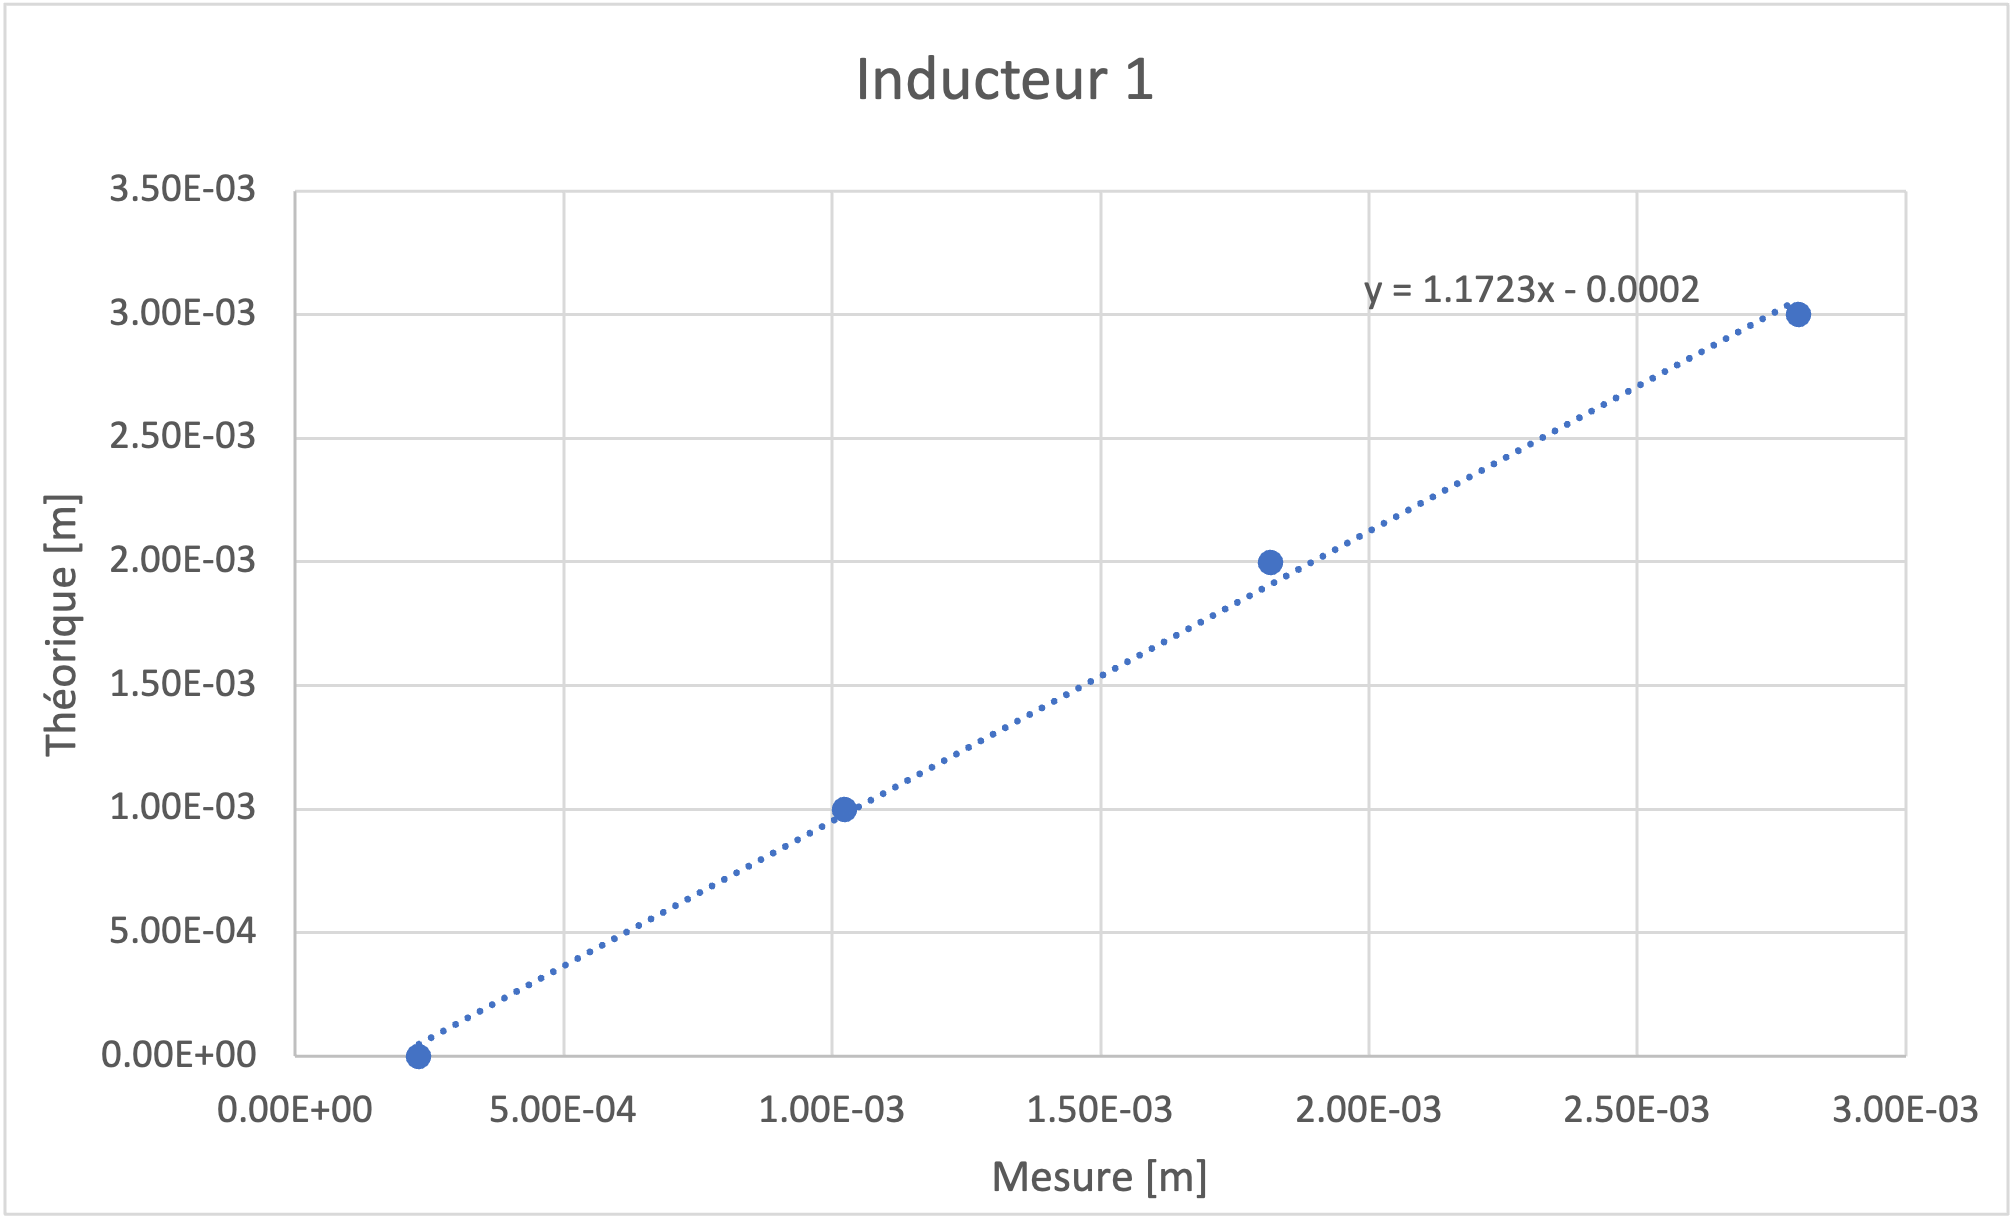
\includegraphics[width=1\linewidth]{assets/Chap3/PremEtaloInd1.png}
    \caption{Graphique de l'étalonnage de l'inducteur 1}
    \label{fig:Prem_tracé_ind1}
\end{figure}

\begin{figure}[H]
    \centering
    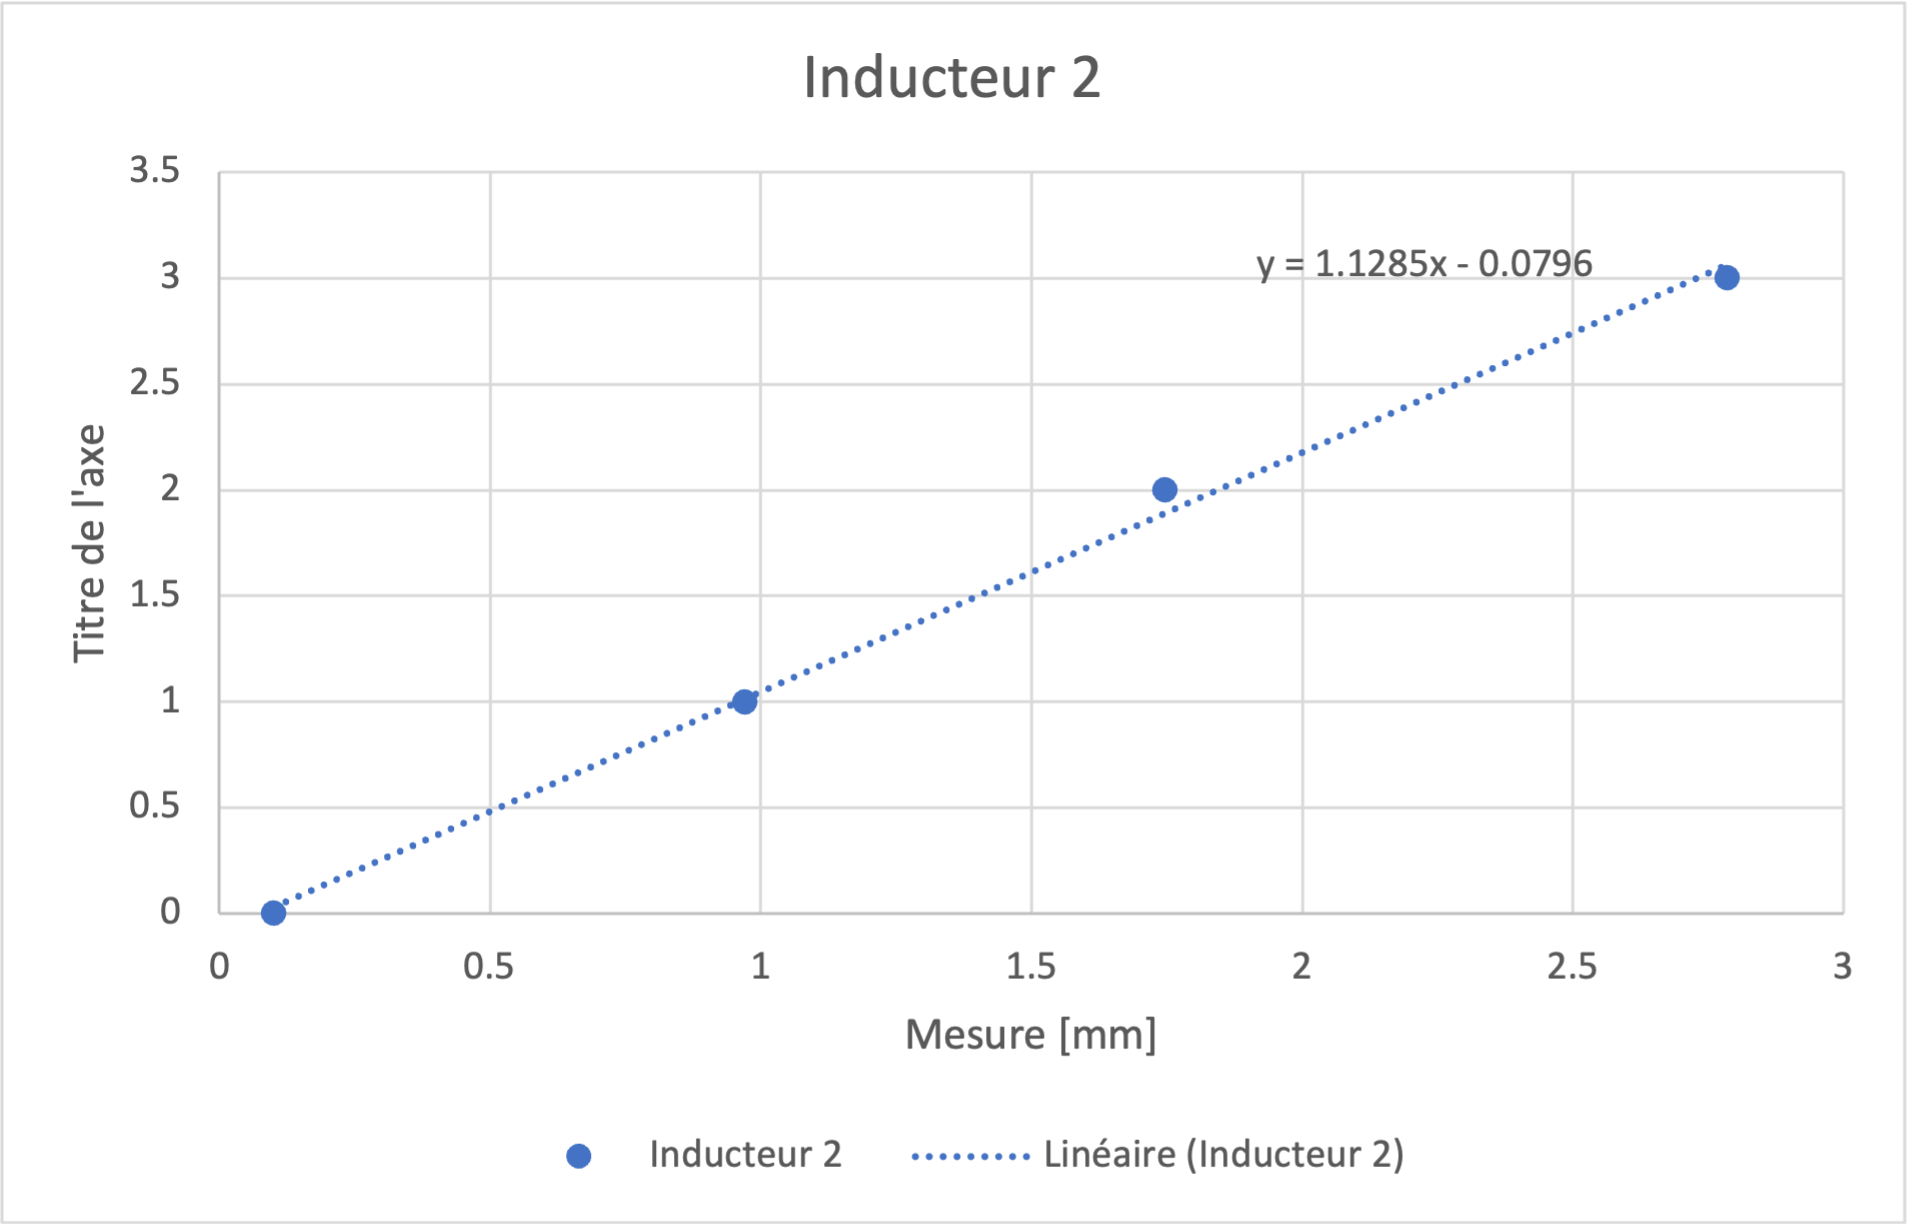
\includegraphics[width=1\linewidth]{assets/Chap3/PremEtaloInd2.png}
    \caption{Graphique de l'étalonnage de l'inducteur 2}
    \label{fig:Prem_tracé_ind2}
\end{figure}

\begin{figure}[H]
    \centering
    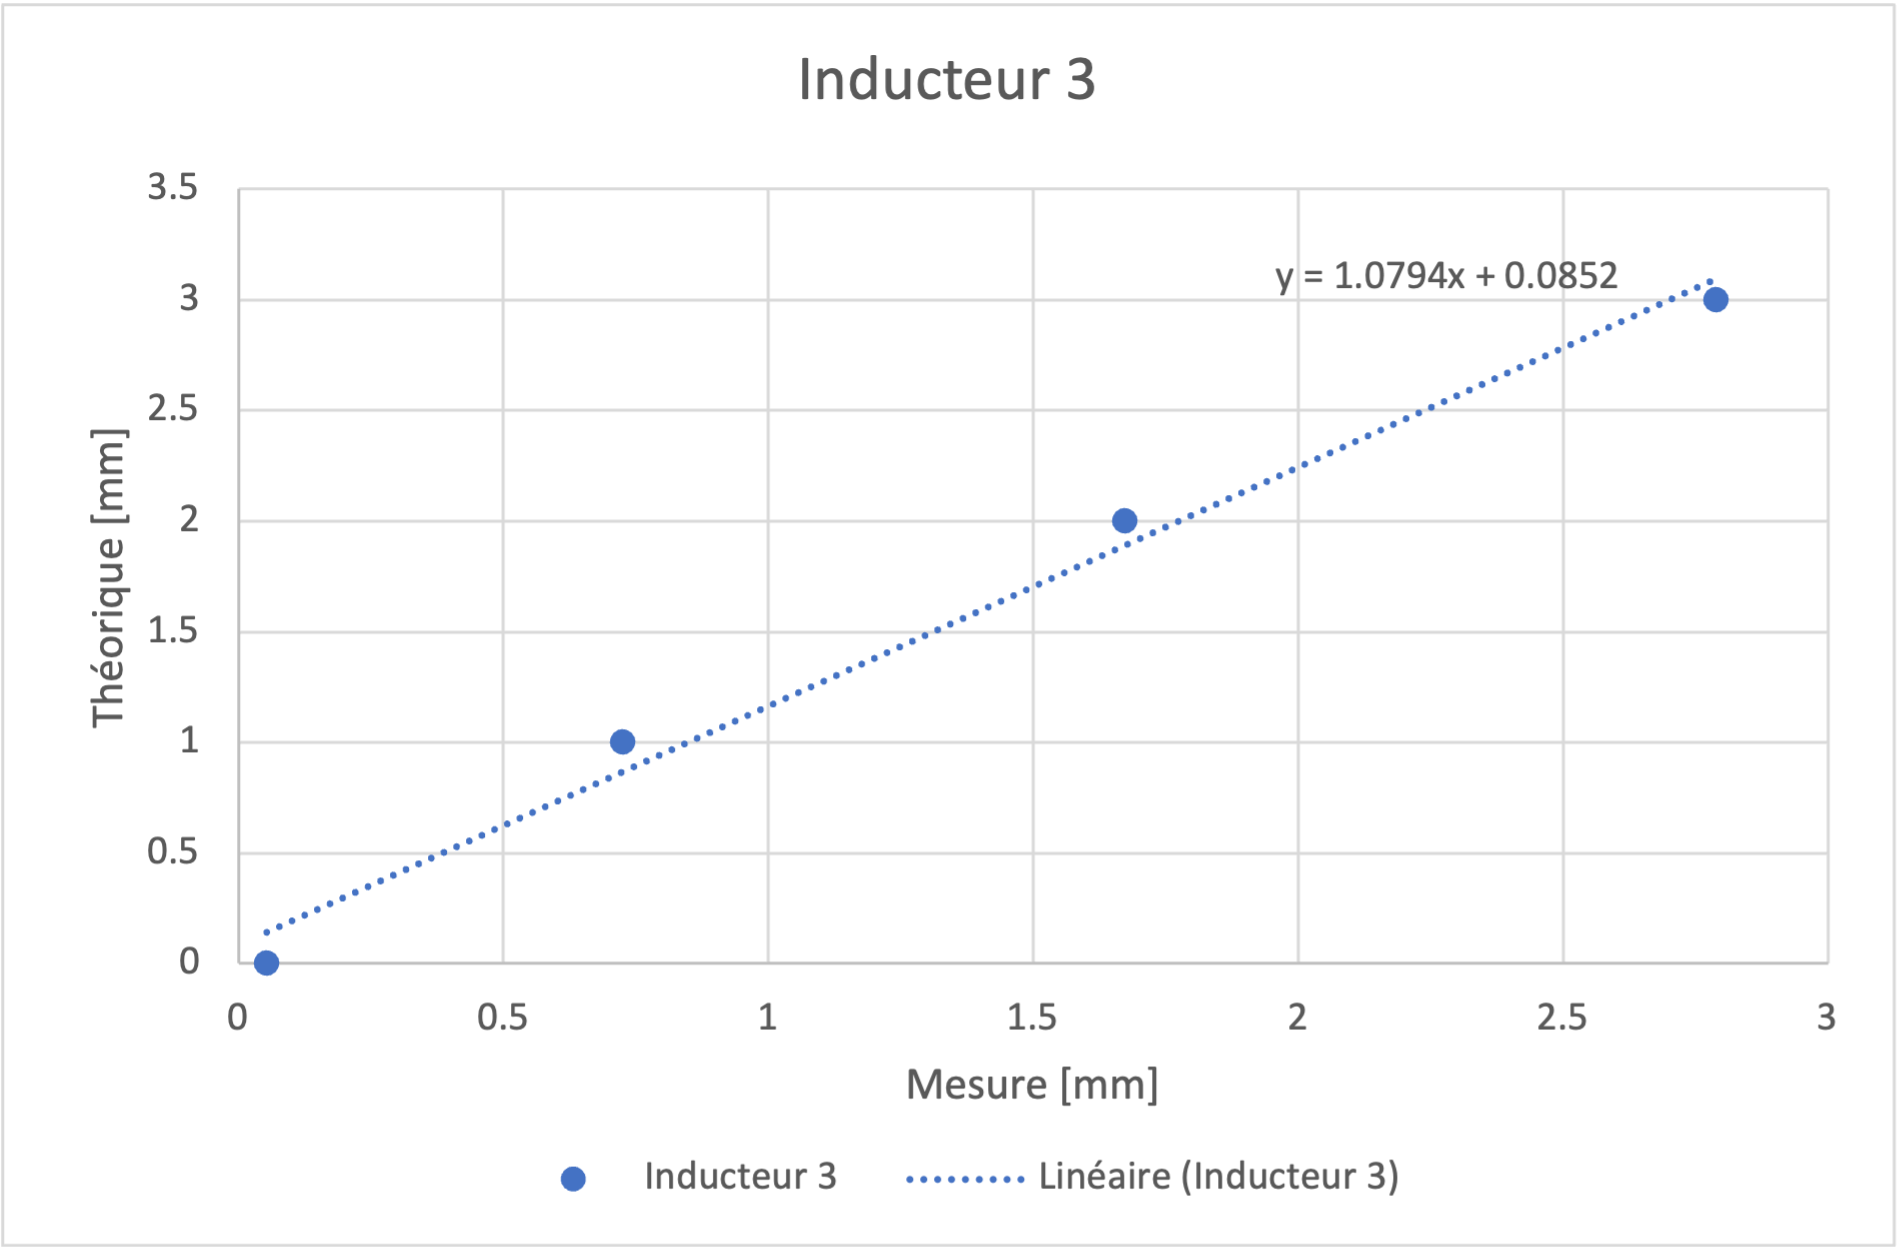
\includegraphics[width=1\linewidth]{assets/Chap3/PremEtaloInd3.png}
    \caption{Graphique de l'étalonnage de l'inducteur 3}
    \label{fig:Prem_tracé_ind3}
\end{figure}

\begin{figure}[H]
    \centering
    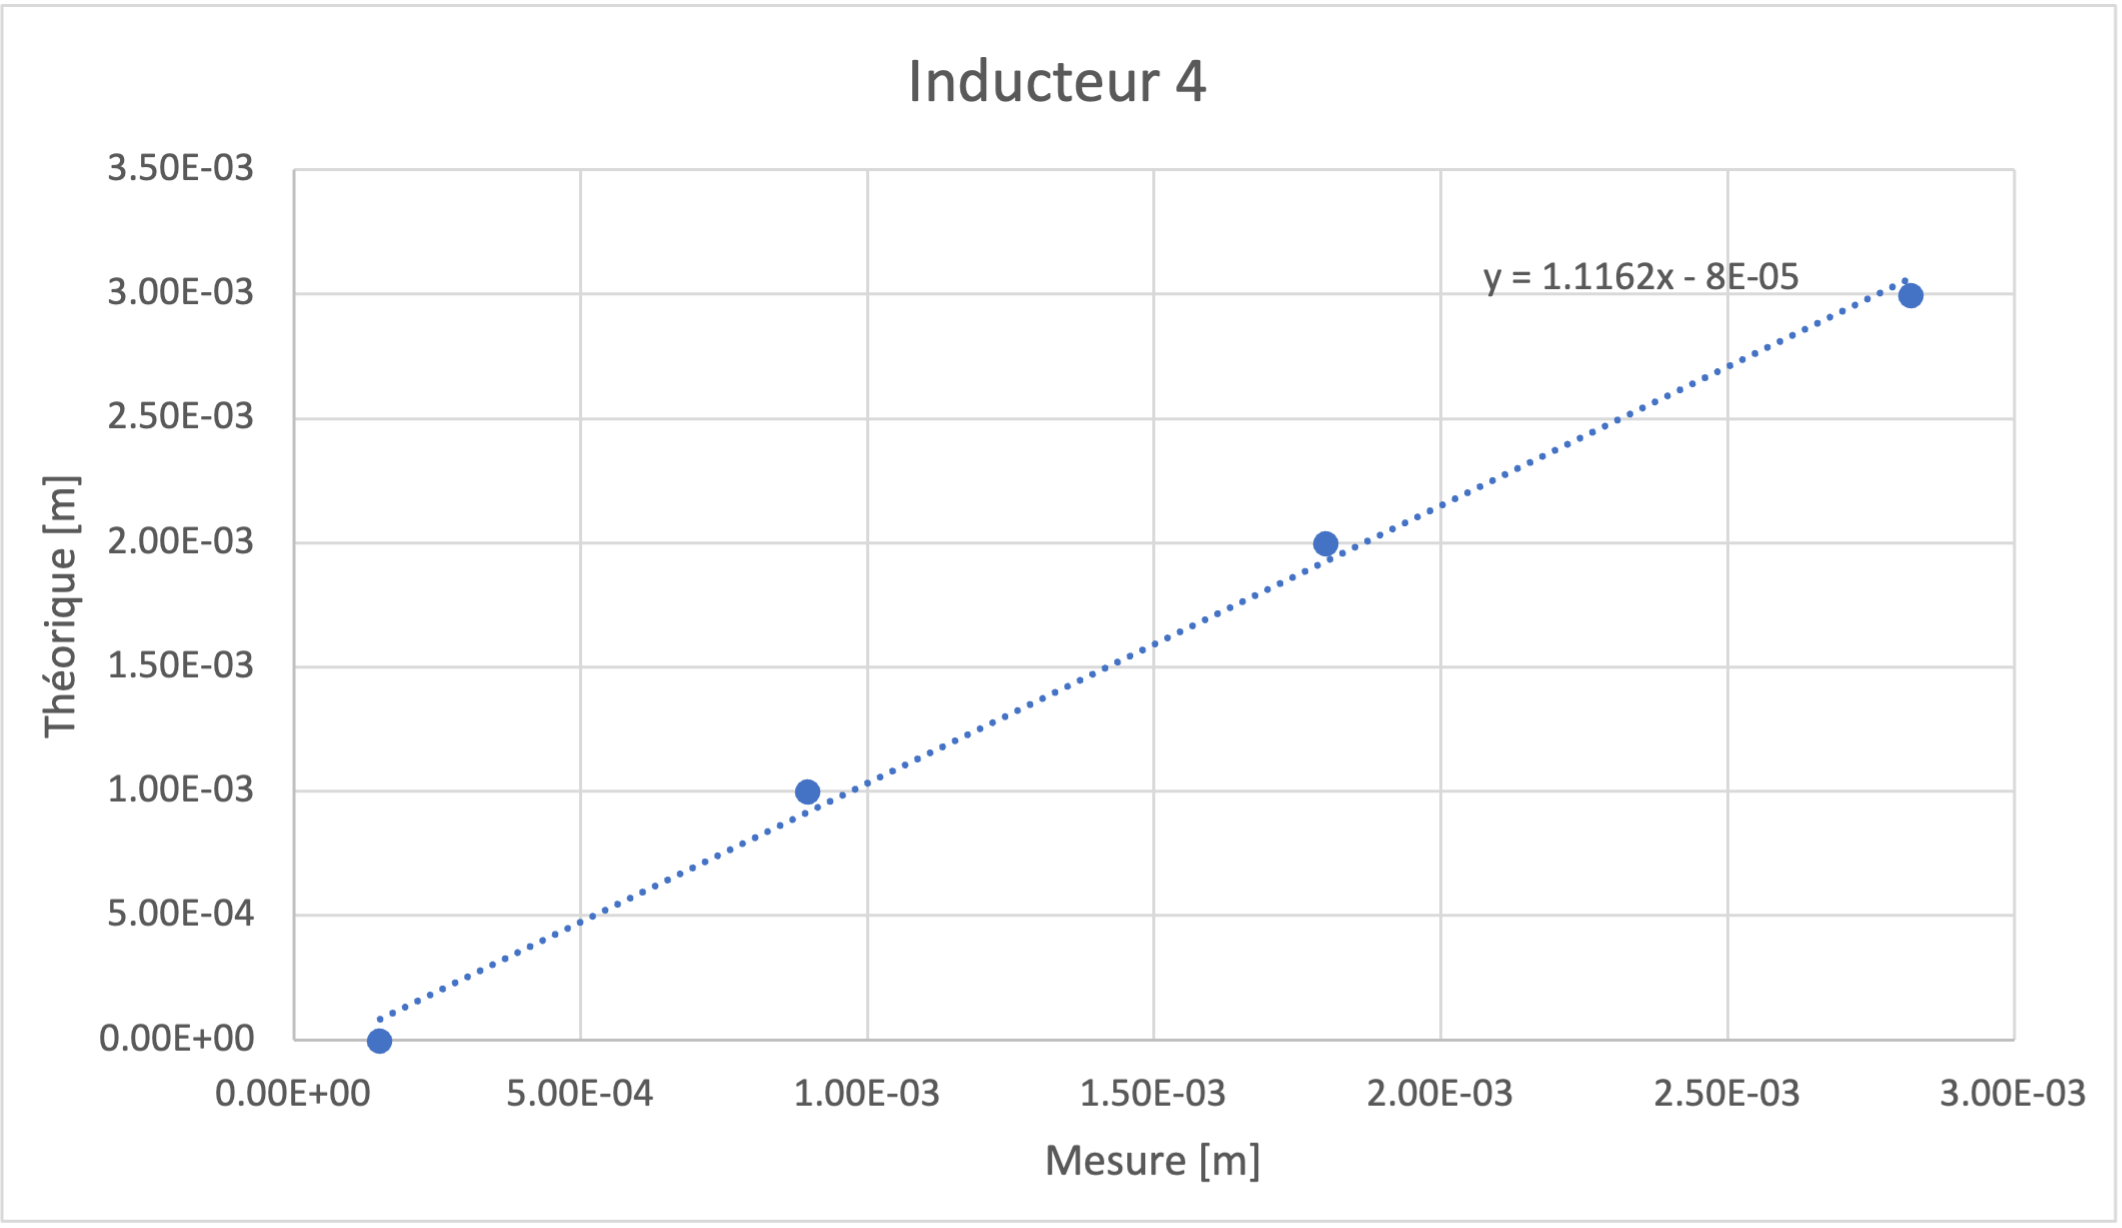
\includegraphics[width=1\linewidth]{assets/Chap3/PremEtaloInd4.png}
    \caption{Graphique de l'étalonnage de l'inducteur 4}
    \label{fig:Prem_tracé_ind4}
\end{figure}

Ces tracé permettent de ressortir des équations permettant d'appliquer une meilleur correction au système avec un gain et un offset, la valeur en x étant la valeur de l'adc convertit en mm.

\subsection{Mesure après la calibration de tous les capteurs}
Lorsque la correction précédente fut appliqué dans le code, le résultat n'était toujours pas convainquant. C'est pour cela qu'une calibration des 4 capteurs fut réalisé. Cela avait pour but d'essayer d'éliminer l'angle qui se créaient par la calibration précédente. La calibration précédente avait réalisé la méthode teach-in en souleant soit l'avant soit l'arrière de la partie lévitante. Meme si très petite, cela crée un angle que l'on peut observer dans la figure suivante :



Afin de palier a cela, les 4 inducteurs ont été soulevé puis abaissé en suivant la démarche expliqué dans la section \ref{sec:CalibrationCaptPos}.

Suite a cette calibration, une nouvelle mesure sans les corrections a été mesuré présent dans le tableau \ref{} :



Cette mesure donna de nouveau lieux à une tentavie de tracé de courbe afin d'obtenir une correction à appliquer dans le code. Ce tracé est observable dans la figure \ref{} :


\subsection{Mesure d'étalonnage des valeurs d'ADC}
Le résultat n'étant toujours pas concluant, il a été décidé d'appliquer une correction immédiatement sur la valeur de l'ADC. Dans le travail de bachelor précédent, la valeur de l'ADC était convertit suivant une règée de 3 comme présente dans l'équation \ref{eq:conv_ADC_mm} :

\begin{equation}
    y = x
    \label{eq:conv_ADC_mm}
\end{equation}

Ceci est juste pour un système linéaire, cependant les capteurs ayant plus un comportement non linéaire, il a été décidé d'appliquer une conversion ainsi qu'une correction directement sur la valeur brute mesuré de l'ADC. Ceci a également l'envie de supprimer les erreurs liées au tolérance présente entre le capteur et la mesure de l'adc afin de la réduire la plus possible. Ceci donne donc les tableaux \ref{}, \ref{}, \ref{} et \ref{} :



Par la suite une moyenne de chacune des valeurs a été réalisé pour obtenir le tableau \ref{}:


Une première tentative fut de réaliser un polynôme d'ordre 5 :


L'équation retenue est alors :
\begin{equation}
    x = x
\end{equation}


Le résultat n'étant pas concluant et ne semble pas laisser a la maquette d'avoir de la liberté, cet ordre fut baissé à un ordre 3 donnant donc le tracé suivant :


Ceci donne l'équation :
\begin{equation}
    x = x
\end{equation}


Le résultat n'étant toujours pas satisfaisant donna alors lieux à un tracé d'ordre 1 ce qui donne :


Donnat alors l'équation :
\begin{equation}
    x = x
\end{equation}

Lors de la mesure pour controler le bon fonctionnement de la correction appliqué, les capteurs furent une nouvelle fois mesuré afin de controller la corection pour chaque polynome. Ceci donne alors les tableaux \ref{}, \ref{} et \ref{} :

\subsection{Analyse des résultats}
La réalisation du capteurs de positions ne fut pas concluant. Théoriquement le procédé semble correcte cependant elle n'a pas donné lieux à une bonne correction lors de l'usage de celui-ci. Inidquant alors que le problème ne vient pas de la calibration du capteurs de positions mais d'autre part.\\

La théorique la plus probable est du à un mauvais placement des pôles. C'est donc pour cela que la régulation fut une nouvelle fois analysé.

\section{Conclusion des mesures}
Dans la grande majorité des cas les mesures offrent des résultats proche de ce qui est attendue. Confirmant le bon fonctionnement de la carte principale fournissant alors les résultats attendues.